\FloatBarrier
\section{Decomposição aditiva do produto}\label{app:decomposition}
A ordem é \emph{horas físicas, eficiência e realocação formal--informal}. Seja $Y_0$ o produto inicial. O primeiro nível intermediário, $Y_H$, aplica novas horas por faixa, mantendo sua eficiência e composição iniciais. O segundo, $Y_E$, atualiza também a eficiência, preservando composição. O último, $Y_1$, permite reotimização formal--informal. $A$ mantém seu valor inicial em todos os níveis.
\begin{equation}\label{eq:app_decomposition}
\underbrace{100\frac{Y_1-Y_0}{Y_0}}_{\Delta Y}
=\underbrace{100\frac{Y_H-Y_0}{Y_0}}_{\text{horas físicas}}
+\underbrace{100\frac{Y_E-Y_H}{Y_0}}_{\text{eficiência}}
+\underbrace{100\frac{Y_1-Y_E}{Y_0}}_{\text{realocação}}.
\end{equation}
Todos os termos têm denominador comum. Interações são incorporadas à margem atualizada por último; a atribuição depende da ordem e não é única. O último termo é contrafactual definido, não resíduo com denominador diferente.
\begin{table}[htbp]
\centering
\caption{Decomposição nacional com a base formal limitada a 44h}
\label{tab:app_decomposition}
\normalsize
\begin{tabular}{@{}llrrrr@{}}
\toprule
Eficiência & Teto & Horas & Eficiência & Realocação & Total \\
\midrule
Bilateral & 40h & $-2{,}24352$ & $0{,}77145$ & $-0{,}20447$ & $-1{,}67655$ \\
Fadiga & 40h & $-2{,}18876$ & $0{,}75249$ & $-0{,}19951$ & $-1{,}63578$ \\
Bilateral & 36h & $-6{,}70703$ & $-0{,}66221$ & $-1{,}02838$ & $-8{,}39762$ \\
Fadiga & 36h & $-6{,}53974$ & $0{,}70661$ & $-0{,}81309$ & $-6{,}64622$ \\
\bottomrule
\end{tabular}
\begin{minipage}{0.96\textwidth}\normalsize
\textit{Notas:} Parcelas em pontos percentuais da variação de produto, todas divididas por $Y_0$. Valores não arredondados somam à variação total. Fadiga é eficiência constante abaixo do pico. $\sigma=1{,}326$, com ponte e cunhas recalibradas por função.
\end{minipage}
\end{table}
% Generated by scripts/generate_assets.py; do not edit.
\begin{table}[!htbp]
\centering
\normalsize
\caption{Níveis intermediários do produto na decomposição nacional}\label{tab:decomposition_levels}
\setlength{\tabcolsep}{4pt}
\begin{tabular}{llrrrr}
\toprule
Função & Teto & $Y_0$ & $Y_H$ & $Y_E$ & $Y_1$ \\
\midrule
Bilateral & 40h & 4,184726 & 4,090841 & 4,123124 & 4,114567 \\
Bilateral & 36h & 4,184726 & 3,904055 & 3,876343 & 3,833309 \\
Acima do pico & 40h & 4,268422 & 4,174997 & 4,207116 & 4,198600 \\
Acima do pico & 36h & 4,268422 & 3,989279 & 4,019440 & 3,984733 \\
\bottomrule
\end{tabular}
\par\smallskip
\begin{minipage}{0.98\linewidth}\normalsize Fonte: simulações nacionais com PNAD 2024T4, base formal limitada a 44h e ponte horária recalibrada. Produto em unidades normalizadas do modelo, com seis casas decimais; não em reais. A ordem é horas físicas, eficiência e realocação formal--informal: $Y_H$ altera somente as horas, $Y_E$ atualiza também a eficiência, mantendo a composição inicial, e $Y_1$ permite a reotimização. As contribuições percentuais são $100(Y_H-Y_0)/Y_0$, $100(Y_E-Y_H)/Y_0$ e $100(Y_1-Y_E)/Y_0$, cuja soma é $100(Y_1-Y_0)/Y_0$. Os cálculos e o CSV usam precisão integral; diferenças aparentes após arredondamento não são resíduos econômicos.\end{minipage}
\end{table}

\begin{figure}[htbp]
\centering
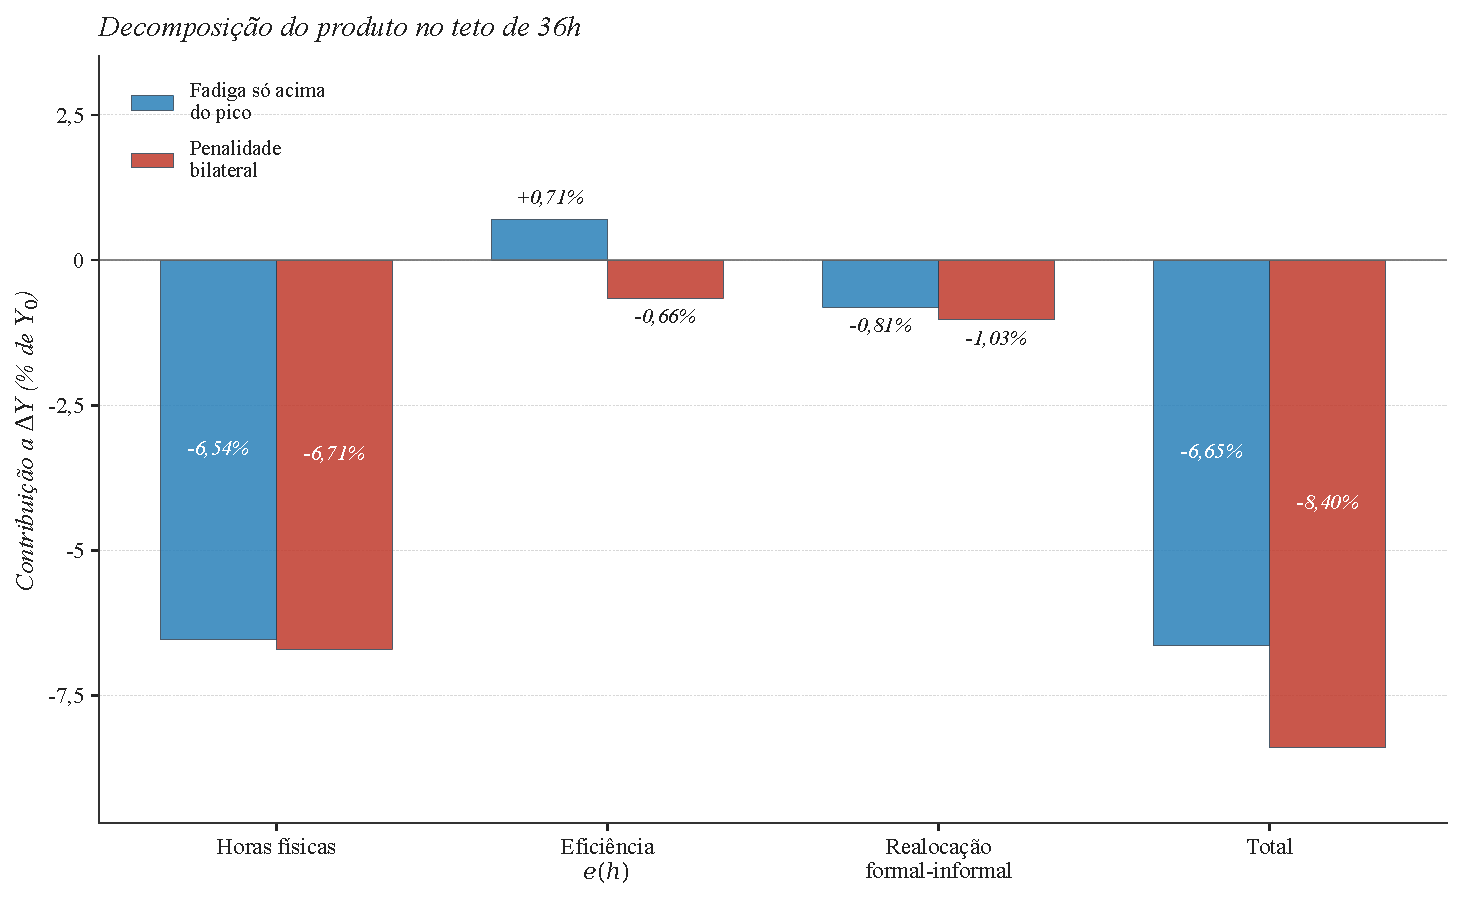
\includegraphics[width=0.96\textwidth]{generated/fig_decomposition.pdf}
\caption{Horas físicas, eficiência e realocação na variação do produto em 36h}
\label{fig:decomposition}
\begin{minipage}{0.96\textwidth}\normalsize
\textit{Notas:} Comparação 44$\to$36h, nas duas funções de eficiência. As três parcelas usam o mesmo denominador $Y_0$ e somam à variação total, na ordem da Equação~\eqref{eq:app_decomposition}, com dados reprocessados e sem compensação exógena. Diferenças entre funções refletem também a calibração da ponte e do estado inicial.
\end{minipage}
\end{figure}

\FloatBarrier
\section{Comparação de versões e sensibilidade}\label{app:sensitivity}\label{app:hours_efficiency}
\subsection{Correções de código e atualização das entradas}
A Tabela~\ref{tab:comparison} separa execução original, núcleo corrigido com entradas congeladas e dados reprocessados. O controle congelado corrige contabilidade, resolve continuamente a composição e recalibra cunhas sob normalização explícita. Pesos de horas, taxas por porte e hipóteses legadas são preservados; isso não valida a origem empírica anteriormente atribuída a eles.

A passagem aos dados reprocessados envolve um grupo nacional e os momentos da distribuição habitual observada. Publicam-se controles intermediários: alteração isolada da participação RAIS, um grupo com entradas congeladas, $\omega=0{,}622$ com novos dados e recalibração da ponte. A versão principal limita a base formal a 44h e recalibra novamente a ponte; a distribuição integral permanece como controle de sensibilidade. Essas etapas impedem atribuir toda a diferença ao erro de CNPJ ou à otimização. Níveis de produto normalizados não devem ser comparados entre tecnologias como crescimento observado.
% Generated by scripts/generate_assets.py; do not edit.
\begin{table}[!htbp]
\centering
\normalsize
\caption{Comparação entre versões: código e hipóteses legadas}\label{tab:comparison}
\setlength{\tabcolsep}{4pt}
\begin{tabular}{lrrrrr}
\toprule
Função e teto & $\Delta Y$ (\%) & $A_{\rm req}$ (\%) & Inf. (\%) & $\Delta GHH$ (\%) & $CE$ (\%) \\
\midrule
\addlinespace
\multicolumn{6}{l}{\textit{Original}} \\
\addlinespace
Bilateral, 40h & -2,00 & 1,92 & 38,16 & 0,41 & 0,32 \\
Bilateral, 36h & -8,02 & 8,18 & 39,62 & -3,63 & -2,84 \\
Acima do pico, 40h & -2,00 & 1,93 & 38,16 & 0,41 & 0,32 \\
Acima do pico, 36h & -6,60 & 6,63 & 39,27 & -1,76 & -1,38 \\
\addlinespace
\multicolumn{6}{l}{\textit{Código corrigido; entradas congeladas}} \\
\addlinespace
Bilateral, 40h & -2,01 & 1,92 & 41,45 & 0,23 & 0,18 \\
Bilateral, 36h & -8,07 & 8,18 & 43,14 & -4,06 & -3,18 \\
Acima do pico, 40h & -2,01 & 1,92 & 41,45 & 0,24 & 0,19 \\
Acima do pico, 36h & -6,63 & 6,62 & 42,73 & -2,17 & -1,70 \\
\addlinespace
\multicolumn{6}{l}{\textit{Ponte horária legada recalibrada}} \\
\addlinespace
Bilateral, 40h & -1,84 & 1,79 & 41,35 & 0,47 & 0,36 \\
Bilateral, 36h & -7,38 & 7,59 & 42,71 & -3,12 & -2,44 \\
Acima do pico, 40h & -1,83 & 1,79 & 41,35 & 0,47 & 0,37 \\
Acima do pico, 36h & -6,06 & 6,15 & 42,38 & -1,39 & -1,09 \\
\addlinespace
\multicolumn{6}{l}{\textit{Somente RAIS verificada}} \\
\addlinespace
Bilateral, 40h & -1,99 & 1,93 & 35,70 & 0,54 & 0,42 \\
Bilateral, 36h & -7,99 & 8,19 & 36,99 & -3,31 & -2,59 \\
Acima do pico, 40h & -1,99 & 1,92 & 35,70 & 0,54 & 0,42 \\
Acima do pico, 36h & -6,56 & 6,63 & 36,68 & -1,45 & -1,14 \\
\bottomrule
\end{tabular}
\par\smallskip
\begin{minipage}{0.98\linewidth}\normalsize Fonte: execução original arquivada e versões explicitadas da replicação corrigida. $\sigma=1{,}326$ em todas as linhas. A versão original é uma nova execução do código preservado; seu $CE$ foi calculado das alocações originais. Informalidade é nível após reforma. As versões intermediárias isolam modificações condicionais e não são todas calibrações empíricas preferidas. Na versão com RAIS, vínculos por estabelecimento são combinados apenas experimentalmente com taxas de informalidade legadas. Os conceitos e denominadores seguem a Tabela~\ref{main-tab:mainresults} do artigo.\end{minipage}
\end{table}

% Generated by scripts/generate_assets.py; do not edit.
\begin{table}[!htbp]
\centering
\normalsize
\caption{Comparação entre versões: agregação e dados reprocessados}\label{tab:comparison_data}
\setlength{\tabcolsep}{4pt}
\begin{tabular}{lrrrrr}
\toprule
Função e teto & $\Delta Y$ (\%) & $A_{\rm req}$ (\%) & Inf. (\%) & $\Delta GHH$ (\%) & $CE$ (\%) \\
\midrule
\addlinespace
\multicolumn{6}{l}{\textit{Controle de um grupo; entradas congeladas}} \\
\addlinespace
Bilateral, 40h & -1,96 & 1,92 & 41,50 & 0,30 & 0,23 \\
Bilateral, 36h & -7,86 & 8,17 & 43,37 & -3,83 & -3,00 \\
Acima do pico, 40h & -1,96 & 1,92 & 41,50 & 0,30 & 0,24 \\
Acima do pico, 36h & -6,46 & 6,62 & 42,91 & -1,98 & -1,55 \\
\addlinespace
\multicolumn{6}{l}{\textit{PNAD reprocessada; $\omega$ fixo}} \\
\addlinespace
Bilateral, 40h & -0,07 & 0,07 & 38,62 & 3,97 & 3,11 \\
Bilateral, 36h & -6,08 & 6,26 & 40,37 & 0,05 & 0,04 \\
Acima do pico, 40h & -0,07 & 0,07 & 38,62 & 3,97 & 3,11 \\
Acima do pico, 36h & -4,54 & 4,60 & 39,90 & 2,03 & 1,59 \\
\addlinespace
\multicolumn{6}{l}{\textit{PNAD integral; sensibilidade e ponte recalibrada}} \\
\addlinespace
Bilateral, 40h & -0,08 & 0,07 & 38,63 & 3,96 & 3,10 \\
Bilateral, 36h & -6,91 & 6,80 & 40,97 & -1,01 & -0,79 \\
Acima do pico, 40h & -0,08 & 0,07 & 38,63 & 3,96 & 3,10 \\
Acima do pico, 36h & -5,17 & 5,00 & 40,35 & 1,22 & 0,96 \\
\addlinespace
\multicolumn{6}{l}{\textit{Principal: PNAD com base 44h e nova ponte}} \\
\addlinespace
Bilateral, 40h & -1,68 & 1,57 & 39,15 & 0,22 & 0,18 \\
Bilateral, 36h & -8,40 & 8,38 & 41,52 & -4,37 & -3,42 \\
Acima do pico, 40h & -1,64 & 1,53 & 39,14 & 0,28 & 0,22 \\
Acima do pico, 36h & -6,65 & 6,52 & 40,88 & -2,12 & -1,66 \\
\bottomrule
\end{tabular}
\par\smallskip
\begin{minipage}{0.98\linewidth}\normalsize Fonte: execução original arquivada e versões explicitadas da replicação corrigida. $\sigma=1{,}326$ em todas as linhas. A versão original é uma nova execução do código preservado; seu $CE$ foi calculado das alocações originais. Informalidade é nível após reforma. As versões intermediárias isolam modificações condicionais e não são todas calibrações empíricas preferidas. Na versão com RAIS, vínculos por estabelecimento são combinados apenas experimentalmente com taxas de informalidade legadas. Os conceitos e denominadores seguem a Tabela~\ref{main-tab:mainresults} do artigo.\end{minipage}
\end{table}



\subsection{Eficiência, pico e distribuição de horas}
A Tabela~\ref{tab:sensitivity} reporta exercícios condicionais com pontos interiores. Variam-se $\varepsilon_q\in\{0{,}4;0{,}6;0{,}8;1\}$, $h^*\in\{38;39;40;41\}$, $\eta_I\in\{0{,}33;0{,}40;0{,}50\}$ e $\sigma\in\{0{,}6;1;1{,}326;1{,}5;2\}$. Ponte e cunhas são recalibradas em cada ponto. Ao alterar o pico, recalcula-se a curvatura mantendo a elasticidade na referência de 42,244h: o exercício muda conjuntamente pico e curvatura sob essa âncora.
% Generated by scripts/generate_assets.py; do not edit.
\begin{table}[!htbp]
\centering
\normalsize
\caption{Sensibilidades condicionais com a ponte horária recalibrada}\label{tab:sensitivity}
\setlength{\tabcolsep}{4pt}
\begin{tabular}{llrrrr}
\toprule
Parâmetro & Valores avaliados & Bil. 40h & Bil. 36h & Acima 40h & Acima 36h \\
\midrule
$E_Q$ & \shortstack[l]{0,4; 0,6\\0,8; 1,0} & 1,15 a 2,40 & 7,42 a 8,85 & 1,11 a 2,40 & 6,08 a 7,42 \\
$h^\star$ & \shortstack[l]{38,0; 39,0\\40,0; 41,0} & 1,50 a 1,69 & 6,55 a 11,60 & 1,48 a 1,53 & 6,25 a 6,52 \\
$\eta_I$ & 0,33; 0,40; 0,50 & 1,57 a 1,57 & 8,38 a 8,38 & 1,53 a 1,53 & 6,52 a 6,52 \\
$\sigma$ & \shortstack[l]{0,600; 1,000\\1,326; 1,500; 2,000} & 1,39 a 1,72 & 7,50 a 9,12 & 1,36 a 1,68 & 5,82 a 7,11 \\
\bottomrule
\end{tabular}
\par\smallskip
\begin{minipage}{0.98\linewidth}\normalsize Fonte: 64 simulações com PNAD 2024T4 e base formal limitada a 44h. As quatro últimas colunas mostram o mínimo e o máximo de $A_{\rm req}$ (\%) entre os valores listados; os pontos individuais estão em \texttt{generated/sensitivity\_empirical.csv}. Cada dimensão varia separadamente, incluindo pontos interiores; as demais hipóteses permanecem na base. A cada ponto, $\omega$ e as cunhas são recalibrados ao mesmo prêmio horário e à informalidade inicial. $E_Q=1$ implica ausência de fadiga. Trata-se de uma grade de sensibilidade, sem interpretação de conjunto identificado.\end{minipage}
\end{table}


A compensação depende da eficiência suposta para as jornadas. Com $\kappa=0$ e base formal limitada a 44h, $\Areq$ é $2{,}397234\%$ em 40h e $7{,}424102\%$ em 36h nas duas funções. CE é $-0{,}670986\%$ e $-2{,}520735\%$, respectivamente. Na sensibilidade com suporte integral, fadiga forte pode gerar compensação negativa em 40h. Essas diferenças impedem interpretar o número central como estimativa causal identificada de ganhos por redução de fadiga.

A distribuição integral muda a base de comparação: $\Areq$ em 40h fica entre $0{,}0721\%$ e $0{,}0739\%$, e em 36h entre $5{,}00\%$ e $6{,}80\%$, abaixo do resultado principal com limitação inicial a 44h. Mantêm-se os microdados, mas mudam transformação inicial e alvo da ponte: a razão com horas formais limitadas a 44h é $1{,}682473$, contra $1{,}622443$ na distribuição integral, com rendimento e horas informais preservados. Alterar o denominador de horas conservando silenciosamente a antiga razão não implementa o mesmo estimando.
% Generated by scripts/generate_assets.py; do not edit.
\begin{table}[!htbp]
\centering
\normalsize
\caption{Horas de base e fadiga: compensação e equivalente de consumo}\label{tab:mapping}
\setlength{\tabcolsep}{4pt}
\begin{tabular}{llrrrr}
\toprule
Cenário & Função & $A_{\rm req}^{40}$ & $CE^{40}$ & $A_{\rm req}^{36}$ & $CE^{36}$ \\
\midrule
Principal: base 44h & Bilateral & 1,57 & 0,18 & 8,38 & -3,42 \\
Principal: base 44h & Acima do pico & 1,53 & 0,22 & 6,52 & -1,66 \\
PNAD integral & Bilateral & 0,07 & 3,10 & 6,80 & -0,79 \\
PNAD integral & Acima do pico & 0,07 & 3,10 & 5,00 & 0,96 \\
Sem fadiga (base 44h) & Bilateral & 2,40 & -0,67 & 7,42 & -2,52 \\
Sem fadiga (base 44h) & Acima do pico & 2,40 & -0,67 & 7,42 & -2,52 \\
\bottomrule
\end{tabular}
\par\smallskip
\begin{minipage}{0.98\linewidth}\normalsize Valores em \%. A limitação inicial a 44h é uma hipótese adicional de mensuração/cumprimento; altera também o denominador da ponte de remuneração horária, que é recalibrada. A base integral preserva todas as horas observadas. A ausência de fadiga mantém a base limitada a 44h e usa $E_Q=1$, $\kappa=0$. Essas alternativas não são observações distintas de horas contratuais.\end{minipage}
\end{table}


\begin{figure}[htbp]
\centering
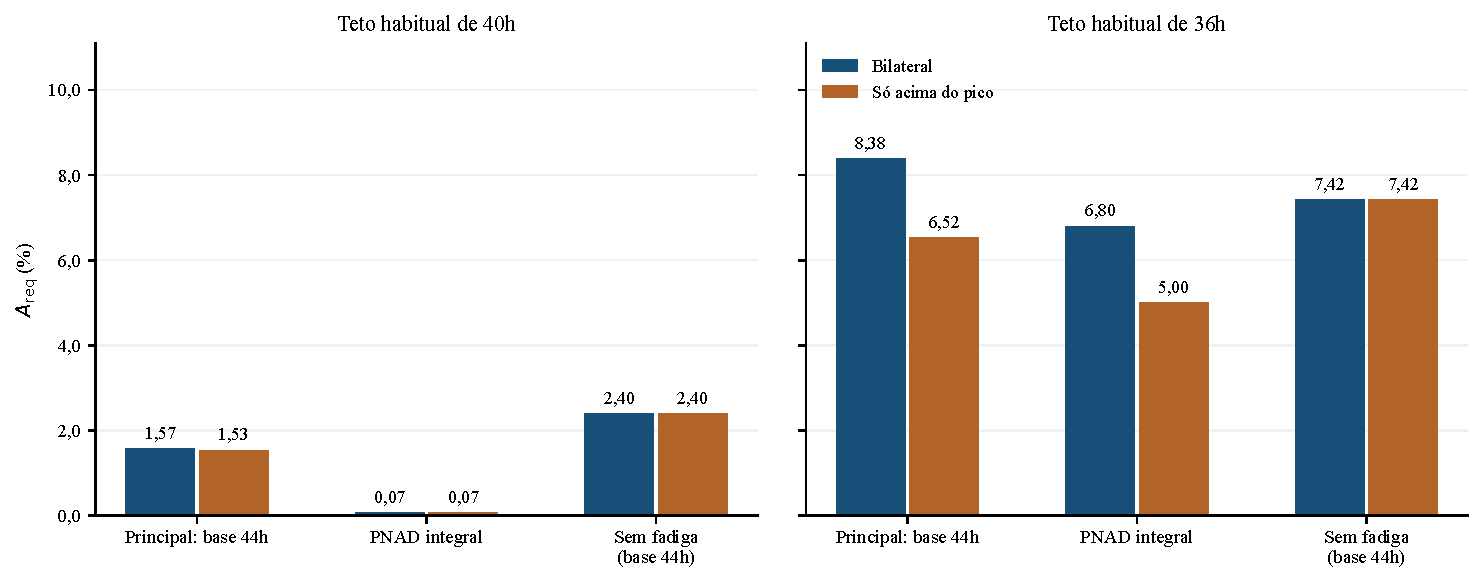
\includegraphics[width=\textwidth]{generated/fig_sensitivity_pt.pdf}
\caption{Sensibilidade da produtividade requerida à eficiência e à distribuição inicial de horas.}\label{fig:sensitivity}
\begin{minipage}{0.96\textwidth}\normalsize
\textit{Notas:} Contrafactuais com os momentos da PNAD 2024T4, recalibrando a ponte horária e as cunhas em cada caso. A base principal limita horas formais a 44h; a distribuição integral é sensibilidade. Sem fadiga, $e(h)=1$. A Tabela~\ref{tab:sensitivity} apresenta as demais sensibilidades, incluindo pontos interiores.
\end{minipage}
\end{figure}


\subsection{CES e limites da interpretação}
Os controles congelados contêm grade conjunta de seis valores de $\sigma$, três de $\omega$ e três de $\eta_I$, além de variações de eficiência, pico e pesos de horas. A grade setorial inclui $3\times3\times3$ combinações, com vértices, faces e ponto interior. São sensibilidades. Uma caixa não é conjunto identificado: seria preciso verificar restrições empíricas em todos os pontos, incerteza amostral e correspondência entre momentos e parâmetros.

Na grade legada, o código registra se a razão horária passa pelo intervalo hipotético $[1{,}15;1{,}55]$, sem presumir que todos os pontos passem. O intervalo não se transporta automaticamente às novas razões amplas: $1{,}622443$ com horas integrais e $1{,}682473$ com horas formais limitadas a 44h, com universo e estimando explícitos. Na grade empírica, ajustar a razão com $\omega$ continua sem identificar separadamente eficiência informal e substituição. Pequena sensibilidade a um parâmetro após recalibrar outro pode refletir compensação entre eles, não precisão empírica do primeiro.

\FloatBarrier
\section{Extensão setorial}\label{app:sectoral}
\subsection{Universo e parâmetros}
A atividade do trabalho principal, CNAE Domiciliar 2.0 (\texttt{V4013}), define agropecuária nas divisões 01--03, indústria e construção em 05--43, serviços em 45--99. As 19.280 pessoas ponderadas não classificáveis são $0{,}018933\%$ dos ocupados e permanecem identificadas no arquivo. A extensão de três setores as exclui explicitamente e normaliza participações entre classificados, cobrindo $99{,}981067\%$ do emprego nacional.
\begin{table}[htbp]
\centering
\caption{Momentos setoriais reprocessados da PNAD 2024T4}
\label{tab:sectoral_params}
\normalsize
\begin{tabular}{@{}lrr@{}}
\toprule
Setor & Ocupados ponderados & Informalidade (\%) \\
\midrule
Agropecuária & 7.712.335,89 & 75,74960 \\
Indústria e construção & 20.848.824,06 & 40,25815 \\
Serviços & 73.251.518,73 & 34,21122 \\
Não classificado & 19.279,83 & 60,02732 \\
\bottomrule
\end{tabular}
\begin{minipage}{0.95\textwidth}\normalsize
\textit{Notas:} Ocupados de 14 anos ou mais, peso V1028. Formalidade usa VD4009 e V4019. As contagens preservam o universo observado; no exercício principal de cada setor, limitam-se as horas habituais formais a 44h antes da calibração. Fonte: \citet{PNAD2024T4Microdados}.
\end{minipage}
\end{table}

Cada setor contém um grupo representativo com emprego e capital fixos. Os pesos de capital $(0{,}0766;0{,}2585;0{,}6649)$ são hipóteses herdadas, originalmente atribuídas a participações de VAB. Mesmo que VAB fosse observado, sua igualdade à participação no capital exigiria outra hipótese. Com $A_g=1$, a composição de produto não é VAB observado. Mantêm-se $\alpha=0{,}35$, $\eta_I=0{,}40$, $\sigma=1{,}326$, $\gamma_g=0{,}06$ e a mesma âncora externa de eficiência.

Calibra-se $\omega$ comum somando folhas e horas dos três setores classificados antes da razão. Com horas formais limitadas a 44h, o alvo é $1{,}682335$, ligeiramente distinto do nacional, $1{,}682473$, pela exclusão das atividades não classificadas também na amostra remunerada. A raiz é $0{,}674476$ na bilateral e $0{,}675575$ na fadiga, distinta da raiz de um grupo. Recalibra-se cada cunha à informalidade setorial. A versão integral com $\omega=0{,}622$ permanece como controle.

\subsection{Resultados e agregação}
% Generated by scripts/generate_assets.py; do not edit.
\begin{table}[!htbp]
\centering
\normalsize
\caption{Resultados setoriais com momentos da PNAD 2024T4}\label{tab:sectoral_results}
\setlength{\tabcolsep}{4pt}
\begin{tabular}{lrrrrrr}
\toprule
Setor & $\Delta Y$ & $A_{\rm req}$ & $A_{\rm req}^{fixo}$ & $\Delta$ Inf. & $\Delta GHH$ & $CE$ \\
\midrule
\addlinespace
\multicolumn{7}{l}{\textit{Bilateral, teto de 40h}} \\
\addlinespace
Agropecuária & -3,08 & 2,09 & 1,90 & 0,82 & -2,44 & -1,91 \\
Indústria e construção & -1,88 & 1,75 & 1,65 & 0,64 & 0,18 & 0,14 \\
Serviços & -1,54 & 1,50 & 1,44 & 0,44 & 0,42 & 0,33 \\
Agregado & -1,71 & 1,60 & 1,51 & 0,51 & 0,18 & 0,14 \\
\addlinespace
\multicolumn{7}{l}{\textit{Bilateral, teto de 36h}} \\
\addlinespace
Agropecuária & -12,06 & 8,85 & 8,03 & 3,21 & -12,06 & -9,44 \\
Indústria e construção & -9,05 & 8,97 & 8,48 & 3,27 & -4,90 & -3,84 \\
Serviços & -7,92 & 8,16 & 7,84 & 2,39 & -3,54 & -2,77 \\
Agregado & -8,42 & 8,41 & 8,00 & 2,63 & -4,39 & -3,44 \\
\addlinespace
\multicolumn{7}{l}{\textit{Só acima do pico, teto de 40h}} \\
\addlinespace
Agropecuária & -3,05 & 2,06 & 1,88 & 0,81 & -2,40 & -1,88 \\
Indústria e construção & -1,87 & 1,73 & 1,64 & 0,64 & 0,20 & 0,15 \\
Serviços & -1,50 & 1,45 & 1,39 & 0,42 & 0,48 & 0,37 \\
Agregado & -1,67 & 1,56 & 1,48 & 0,50 & 0,23 & 0,18 \\
\addlinespace
\multicolumn{7}{l}{\textit{Só acima do pico, teto de 36h}} \\
\addlinespace
Agropecuária & -9,88 & 7,10 & 6,44 & 2,63 & -9,26 & -7,25 \\
Indústria e construção & -7,31 & 7,12 & 6,74 & 2,61 & -2,66 & -2,09 \\
Serviços & -6,22 & 6,31 & 6,06 & 1,84 & -1,37 & -1,07 \\
Agregado & -6,68 & 6,56 & 6,24 & 2,06 & -2,16 & -1,69 \\
\bottomrule
\end{tabular}
\par\smallskip
\begin{minipage}{0.98\linewidth}\normalsize Fonte: PNAD 2024T4 reprocessada; todas as colunas em \%, exceto informalidade em pontos percentuais. Base formal limitada a 44h; horas informais preservadas. O capital setorial e os parâmetros tecnológicos são hipóteses; $\sigma=1{,}326$. A ponte soma folhas e horas entre os três setores classificados, com horas formais limitadas a 44h e $\omega=0,674476$ (bilateral) e $0,675575$ (acima). O agregado recompõe a soma dos produtos com multiplicador comum de produtividade; não é a média dos $A_{\rm req}$ setoriais. Os 0,019\% de ocupados sem atividade classificável são excluídos e as participações são renormalizadas. Capital e ocupação setoriais são fixos; os resultados não incorporam relações insumo-produto.\end{minipage}
\end{table}

O agregado soma produtos e resolve a restauração com produtividade comum, reotimizando as três composições. Sua compensação não é a média simples das setoriais. A heterogeneidade de horas, emprego, capital e eficiência impede exigir coincidência com o modelo nacional de um grupo.

Para 40h, $\Areq$ bilateral é $2{,}0854\%$ na agropecuária, $1{,}7461\%$ na indústria e $1{,}4951\%$ nos serviços; agregadamente, $1{,}6015\%$. Para 36h, é $8{,}8540\%$, $8{,}9691\%$ e $8{,}1616\%$, com agregado $8{,}4051\%$. Na fadiga, em 36h, é $7{,}1044\%$, $7{,}1235\%$ e $6{,}3090\%$, com agregado $6{,}5600\%$. Todos esses resultados comparam o novo teto à base formal limitada a 44h.
\begin{figure}[htbp]
\centering
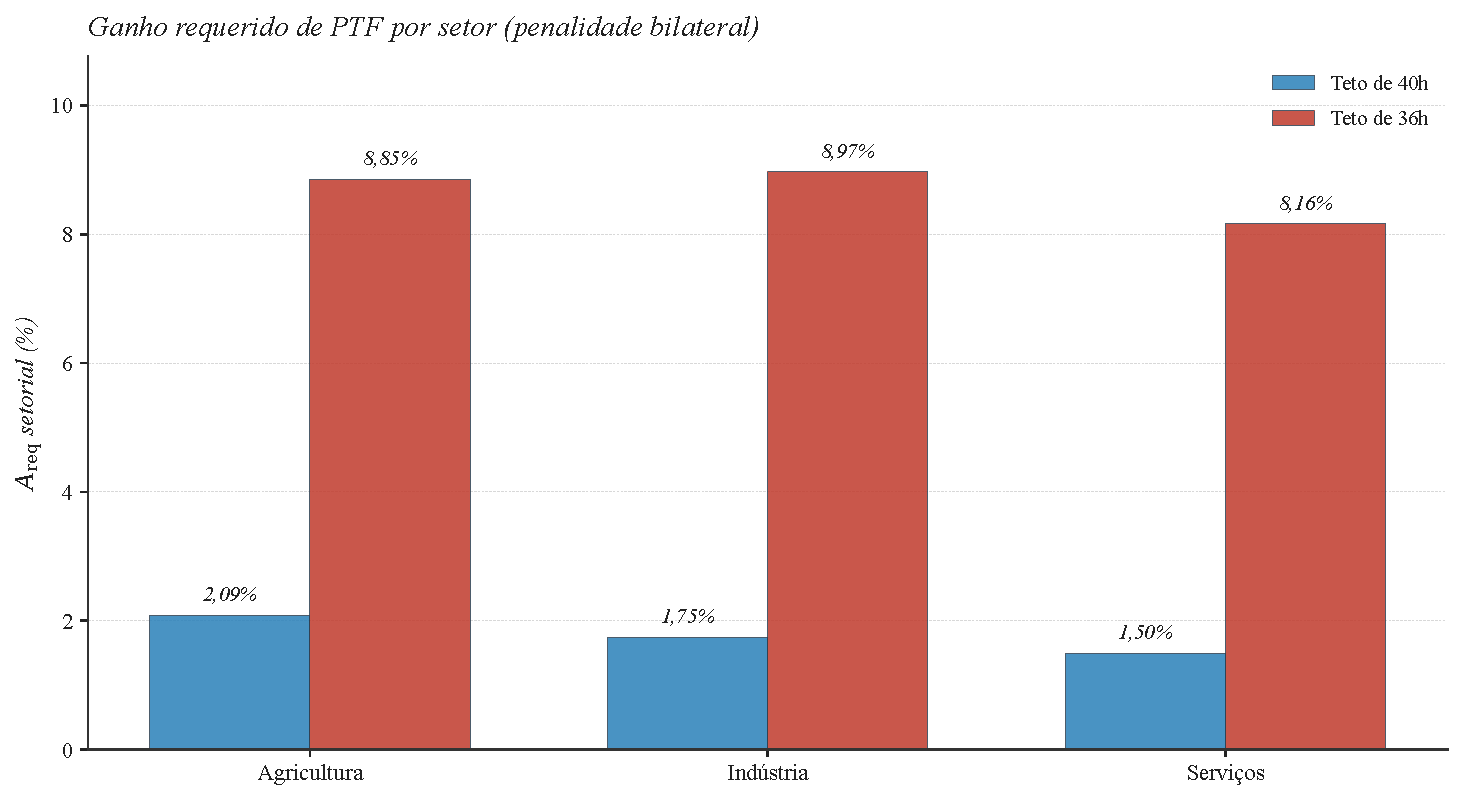
\includegraphics[width=0.96\textwidth]{generated/fig_sectoral_areq.pdf}
\caption{Compensação de produtividade por setor nos tetos de 40h e 36h}
\label{fig:sectoral_areq}
\begin{minipage}{0.96\textwidth}\normalsize
\textit{Notas:} Penalidade bilateral, PNAD 2024T4 reprocessada, base formal limitada a 44h, $\sigma=1{,}326$ e ponte agregada recalibrada. Compensação com sinal e reotimização por setor. A Tabela~\ref{tab:sectoral_results} apresenta também a outra função e o agregado, cuja raiz é resolvida conjuntamente.
\end{minipage}
\end{figure}

Diferenças setoriais não identificam efeitos causais ou política ótima de exceções. Não há mobilidade intersetorial, insumo-produto ou heterogeneidade simultânea por porte e setor. Contagens acima do teto medem exposição mecânica nas horas habituais; não identificam emprego criado, perda individual ou incidência de bem-estar.

\FloatBarrier
\section{Produtividade histórica e horizontes}\label{app:tfp_history_table}
A série brasileira \texttt{rtfpna} da PWT 11.0, arquivada pela série FRED \texttt{RTFPNABRA632NRUG}, fornece referência de escala \citep{PWT2025,FREDPWTBrazil2026}. Usam-se taxas geométricas entre anos disponíveis. Para ganho cumulativo $a-1=\Areq$, expresso como fração, a taxa anual constante equivalente em $T$ anos é
\begin{equation}\label{eq:app_annualized}
g_T=100\left[(1+\Areq)^{1/T}-1\right].
\end{equation}
Ela não é $100\Areq/T$ exceto aproximadamente para pequenas variações. A Tabela~\ref{tab:tfp_horizons} aplica a transformação aos resultados atuais e declara o período histórico.
% Generated by scripts/generate_assets.py; do not edit.
\begin{table}[!htbp]
\centering
\normalsize
\caption{Anualização contábil da compensação de produtividade}\label{tab:tfp_horizons}
\setlength{\tabcolsep}{4pt}
\begin{tabular}{llrrrr}
\toprule
Função & Teto & $A_{\rm req}$ (\%) & 3 anos & 5 anos & 10 anos \\
\midrule
Bilateral & 40h & 1,573 & 0,521 & 0,313 & 0,156 \\
Bilateral & 36h & 8,381 & 2,719 & 1,623 & 0,808 \\
Acima do pico & 40h & 1,534 & 0,509 & 0,305 & 0,152 \\
Acima do pico & 36h & 6,524 & 2,129 & 1,272 & 0,634 \\
\bottomrule
\end{tabular}
\par\smallskip
\begin{minipage}{0.98\linewidth}\normalsize Os ganhos anuais em \% são $g_T=100[(1+A_{\rm req})^{1/T}-1]$, com $A_{\rm req}$ em fração. Base: horas formais limitadas a 44h. A anualização apenas expressa a mesma diferença de nível em outra escala; não é uma trajetória dinâmica estimada. Na PWT 11.0 via FRED, o crescimento anualizado de produtividade do Brasil foi -0,83\% em 1990--2023. Entre janelas de dez anos inteiramente contidas em 1990--2019, a maior taxa foi 0,05\% em 2000--2010. A série serve como referência descritiva de escala e não valida o contrafactual.\end{minipage}
\end{table}


Anualização torna escalas comparáveis; não fornece trajetória de produtividade, nem atribui crescimento à reforma ou garante disponibilidade causal do ganho histórico para financiá-la. Tampouco converte o modelo estático em previsão para três, cinco ou dez anos. A referência PWT difere do canal $e(h)$: somar o mesmo ganho à produtividade exógena e ao trabalho efetivo contaria duas vezes o mecanismo.

\FloatBarrier
\section{Verificação numérica e reprodução}\label{app:replication}
Os dados, controles e resultados nacionais com base limitada a 44h provêm da execução \path{20260905_005724_846373}, concluída integralmente. O pacote registra comandos, versões, entradas, parâmetros, logs e hashes. Código e resultados anteriores foram arquivados antes das alterações. A execução original em saída vazia encontrou uma dependência setorial não gerada pelo antigo orquestrador; as simulações originais do comparativo foram reexecutadas com código arquivado, em processo separado. Figuras antigas não foram consideradas evidência de reprodução.

A reprodução integrada usa, a partir de \path{replication_package}:
\begin{quote}\normalsize
\verb|python run_all.py --refresh-data --tests --paper|
\end{quote}
A reconstrução documental usa \texttt{python build\_paper.py}, a partir de \path{PAPER}. O comando lê arquivos verificados dessa execução e recalcula os exercícios setoriais, a sensibilidade com base limitada a 44h e as curvas adicionais pelo núcleo comum. Também regenera tabelas e figuras e compila os documentos, registrando origens, parâmetros e verificações em \path{generated/ASSET_MANIFEST.json}. As distribuições integrais permanecem nos arquivos de sensibilidade e nos controles de comparação.

Os 61 testes do pacote verificam conversão formal/total, dados e pesos, limites CES, condições de primeira ordem, otimizador independente, cunhas, ponte, restauração, composição congelada, decomposição, recursos e definição de CE. A auditoria da execução de referência verificou 195 hashes e 48 simulações com 264 alocações: maior erro relativo de restauração $2{,}14\times10^{-13}$; maior discrepância de decomposição $5{,}33\times10^{-15}$ pontos percentuais. Nos 80 exercícios adicionais com base limitada a 44h, os maiores erros são $7{,}11\times10^{-15}$ na restauração e $1{,}78\times10^{-15}$ pontos percentuais na decomposição; as âncoras nacionais reproduzem o arquivo canônico.

São controles computacionais e contábeis. Recuperar pesos, médias de horas e taxas usados na calibração não é validação comportamental externa. Resultados dependem de eficiência, remuneração competitiva, recursos, preferências e alcance do teto. Evidências de outras reformas contextualizam mecanismos, mas não identificam automaticamente os parâmetros nem eliminam limitações de universo e mensuração.
